\chapter{Finite Markov Decision Process}

\section{Summary}

MDP's are a formal framework to model sequential decision making. It can handle immediate and delayed rewards, incorporating state.

\subsection{Agent-Environment Interface}

\begin{enumerate}
	\item agent: Leaner and decision maker.
	\item environment: The thing the agent interacts with.
	\item $P(s', r|s,a)$: dynamics of the system (as probability distribution) 
\end{enumerate}

If the next state $S_{t+1}$ only depends on the current state $S_t$ and the input $A_t$, then the state is said to have the \textbf{Markov property} .

\begin{figure}[H]
	\centering
	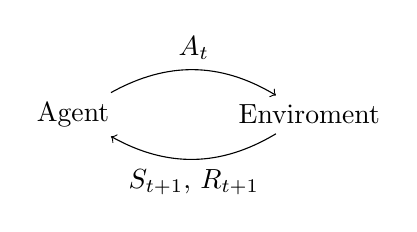
\begin{tikzpicture}
	
	\node at (1, 0) (a) {Agent};
	\node at (4, 0) (b) {Enviroment};
	
	\draw [->, auto, bend left] (a) to node {$A_t$} (b);
	\draw [->, auto, bend left] (b) to node {$S_{t+1}$, $R_{t+1}$} (a);
	\end{tikzpicture}
	\caption{Agent Environment}
	\label{fig:agent-enviroment}
\end{figure}

\subsection{Goals and rewards}

The \textbf{reward hypothesis} say's that all goals/purposes can be expressed as maximizing reward.

Reward should only communicate \textbf{what} needs to be done, not \textbf{how}.

\subsection{Returns and episodes}
An \textbf{episodial task} has a finite number of steps, until it stops in the absorbing state. $G_t = R_{t+1} + R_{t+2} + ... + R_{T}$.

A \textbf{continuing task} never stops, so it keeps getting rewards. So an extra concept \textbf{discount factor}($\gamma$) is needed to define the expected reward.  

\begin{equation}
\begin{split}
G_T & = R_{t+1} + \gamma R_{t+2} + ... \\
& = \sum_{k=0}^{\infty}\gamma R_{t+k+1} \\
& 0 \leq \gamma \leq 1
\end{split}
\label{eq:expected return continuing task}
\end{equation}

The discount factor is a geometric series, and equals to one.
\begin{equation}
\sum_{k=0}^{\infty} \gamma ^k = \frac{1}{1-\gamma}
\label{eq:discount factor geometry series}
\end{equation}

\subsection{Policies and value function}
The \textbf{state-value function} expressed how it is to be in a certain state under a certain policy($\pi$). It has a recursive definition that is derived in equation~\ref{eq:bellman equation value function derivation} and known as the \textbf{bellman equation}.

\begin{equation}
\begin{split}
V_{\pi}(s) & = \EX\left[G_t | S_t = s\right]\\
& = \EX\left[\sum_{k=0}^\infty \gamma^k R_{t + k + 1} | S_t = s\right]\\
& = \EX\left[R_{t+1} + \gamma G_{t+1} | S_t = s \right]\\
& = \sum_a \pi(a|s)\sum_{s',r} p(s', r|s,a)( r + \gamma \EX_\pi[G_{t+1}|S_{t+1}=s']) \\
& = \sum_a \pi(a|s)\sum_{s',r} p(s', r|s,a)( r + \gamma v_\pi(s'))
\end{split}
\label{eq:bellman equation value function derivation}
\end{equation}

The value of taking action $a$ under state $s$ is defined by the \textbf{action-value function} equation~\ref{eq:action-value function}.

\begin{equation}
\begin{split}
q_\pi(a, s) 
& = \EX[G_t | S_t = s, A_t = a]\\
& = \EX\left[\sum_{k=0}^\infty \gamma^k R_{t + k + 1} | S_t = s, A_t = a\right]\\
& = \sum_{r,s'} p(s', r|s,a)( r + \gamma v_\pi(s'))
\label{eq:action-value function}
\end{split}
\end{equation}

\subsection{Optimal policies and optimal value function}
Solving a \textbf{reinforcement learning} problem is finding a policy that gets a lot of reward. The best possible policy is called the \textbf{optimal policy}, the value-state function of this policy is the \textbf{optimal state-value function} $v_*(s)=\max_{\pi}v_\pi(s)$. And the action-value function is the \textbf{optimal value-state function} $q_*(s, a)= \max_{\pi} q_\pi (s, a)$ 

\begin{equation}
\begin{split}
v_* 
& = \max_a q_\pi (s, a) \\
& = \max_a \EX\left[ G_t | S_t=a, A_t=a \right] \\
& = \max_a \EX\left[ R_{t+1} + \gamma G_t | S_t=a, A_t=a \right] \\
& = \max_a \EX\left[ R_{t+1} + \gamma V_*(S_{t+1}) | S_t=a, A_t=a \right] \\
& = \max_a \sum_{s}p(s', r | a, s) [r+ \gamma V_*(s')] \\
\end{split}
\label{eq:bellman optimality equation state-value function derivation}
\end{equation}

The optimal state-value and action-value functions lead to \textbf{the bellman optimality equations} equation~\ref{eq:bellman optimality equation state-value function derivation} and equation~\ref{eq:bellman optimality equation action-value function derivation}

\begin{equation}
\begin{split}
q_*(s, a) 
& = \EX\left[ R_{t+1} + \gamma \max_{a'} q(S_{t+1},a') | S_t=s, A_t=a \right] \\
& = p(s' r | s, a)[ r + \gamma \max_{a'} q(s', a)]
\end{split}
\label{eq:bellman optimality equation action-value function derivation}
\end{equation}

\section{Exercises}

\subsection{Exercise 3.1}
A Robot in a maze has a delayed reward, and needs to make a sequence of decisions. The position of the robot in the maze is the state, and the input is the decisions left/right/straight ahead. The reward is -1 until the absorbing state, which has a reward of zero.

A automatic poker player can be a mdp, the state is the current cards in the hand and the table. 